\documentclass[]{jsarticle}
\usepackage[dvipdfmx]{graphicx}
\usepackage{comment}
\usepackage{float}

\usepackage{listings,jvlisting}
\lstset{
  basicstyle={\ttfamily},
  identifierstyle={\small},
  commentstyle={\smallitshape},
  keywordstyle={\small\bfseries},
  ndkeywordstyle={\small},
  stringstyle={\small\ttfamily},
  frame={tb},
  breaklines=true,
  columns=[l]{fullflexible},
  numbers=left,
  xrightmargin=0zw,
  xleftmargin=2zw,
  numberstyle={\scriptsize},
  stepnumber=1,
  numbersep=1zw,
  lineskip=-0.5ex,
}

\title{\textbf{課題5:学習用アプリ\\(WordMaster: PWT-R Edition)}}
\author{\textbf{I類 メディア情報学 LEORA DAVID}\\\textbf{学籍番号}:2210745}

\date{\today}


\begin{document}

\maketitle

\newpage
\tableofcontents
\newpage

\section{はじめに}

このレポートは、「WordMaster: PWT-R Edition」という学習用アプリの開発過程とその機能について説明するものである。本アプリは、英語の授業「Technical English - Basic English for Science」で実施される試験、「Program-Wide Test-Reading (PWT-R) 100-word list」の単語を効率的に学習するために設計された。特に、100 Wordsの試験に備えるための一つの対策手段として、学習者が単語の意味を覚え、語彙力を強化することを目的としている。本レポートでは、アプリの目的、機能、使い方、学習者からのイベント群、および実行例を詳しく説明する。
全ての機能はHTML、CSS、JavaScriptを1枚のHTMLファイルに書き、各機能を別々のコンテナーで表示することで実装した。そうすることで、学習者が各機能に移動する際に、ページの再読み込みをする必要がなく、スムーズに学習を進めることができる。
また、学習の際に、勉強の気合を入れるために、アプリの背景には、勉強に集中するための緑色の背景を使用した。また、ボタンのデザインは、学習者が使いやすいように、大きくて分かりやすいデザインを採用した。全体的に、シンプルで使いやすいデザインを心がけ、学習者がストレスなく学習を進めることができるように設計した。

\section{アプリの目的}

このアプリの目的は、英語の語彙力を強化することである。特に、「Technical English - Basic English for Science」の授業で使用されるPWT-R 100-word listに含まれる単語の意味を効率的に覚えるためのツールとして、クイズ形式で学習を進めることを支援する。学習者が単語の意味を確認し、正しい単語を選択することで、語彙の定着を図ることができる。また、テストに備えるための対策手段として、いつでもどこでも学習できるようにすることを目指している。\\
\newline
また、誰でもどこでもアクセスできるように、Amazon S3を使用してアプリをデプロイし、URLを共有した。URLは以下の通りである:\\
\textbf{URL:} \textit{http://wordmaster-pwtr-edition.s3-website-us-east-1.amazonaws.com/}

\newpage
\section{アプリの機能}

本アプリは、以下の主要な機能を備えている:

\subsection{クイズ機能}
\begin{itemize}
    \item ランダムに選ばれた単語の意味を表示し、学習者が4つの選択肢から正しい単語を選ぶクイズ形式の学習モードである。
    \item クイズの問題数を選択できる機能があり、学習者は自分の学習ペースに合わせて問題数を調整できる。
    \item 正解した問題は再度出題されないが、不正解の問題は再度出題されるため、復習効果を高める。
\end{itemize}

\subsection{フラッシュカード機能}
\begin{itemize}
    \item 単語とその意味を順番に表示し、効率的な復習をサポートする機能である。
    \item 「Show Answer」ボタンをクリックすることで、答えを表示したり隠したりできる。
    \item 「Next」および「Prev」ボタンを使用して前後のカードに移動できる。
\end{itemize}

\subsection{全単語リスト表示機能}
\begin{itemize}
    \item PWT-R 100-word listの全単語とその意味を一覧で確認できる。
    \item 学習者が一目で全単語を確認できるため、全体の把握や復習に役立つ。
\end{itemize}

\newpage
\section{使い方}

本アプリの使い方は以下の通りである:

\subsection{ホーム画面}
ホーム画面には、「Start Quiz」、「Flashcards」、「Show All Words」の3つのボタンがある。「Start Quiz」ボタンをクリックすると、クイズモードが開始される。学習者は問題数を選択することができ、選択した問題数に基づいてクイズが出題される。次に、「Flashcards」ボタンをクリックすると、フラッシュカードモードが開始される。学習者は単語とその意味を順番に確認しながら学習を進めることができる。最後に、「Show All Words」ボタンをクリックすると、全単語リストが表示される。学習者は全ての単語とその意味を一度に確認することができる。

\subsection{クイズモード}
クイズモードでは、画面に単語の意味が表示され、学習者は4つの選択肢から正しい単語を選ぶ。正しい単語を選択すると、「Correct!」というフィードバックが表示される。不正解の場合は、「Incorrect! The correct answer is '単語'」というフィードバックが表示される。回答後、「Next」ボタンをクリックして次の問題に進む。クイズが終了すると、総合スコアが表示される。クイズが始まると最後まで回答しなければならいので注意が必要である。(再読み込みするのであれば仕方ない)

\subsection{フラッシュカードモード}
フラッシュカードモードでは、単語とその意味が順番に表示される。「Show Answer」ボタンをクリックすると、単語の意味が表示され、もう一度クリックすると意味が隠れる。「Next」ボタンをクリックすると次のカードに進み、「Prev」ボタンをクリックすると前のカードに戻る。

\subsection{全単語リスト}
「Show All Words」ボタンをクリックすると、PWT-R 100-word listの全単語とその意味が一覧表示される。「Back to Home」ボタンをクリックすると、ホーム画面に戻る。\\
\newline
\textbf{実装仕方を分かりやすくするために、以下の「実行例」に画像を添付して説明する。}

\newpage
\section{学習者からのイベント群}

学習者からの主なイベントは以下の通りである:

\subsection{選択肢の選択}
学習者がクイズモードで4つの選択肢の中から1つをクリックするイベントである。正解の場合、「Correct!」というフィードバックが表示され、不正解の場合は「Incorrect! The correct answer is '単語'」というフィードバックが表示される。

\subsection{次の問題へ移動}
クイズモードで「Next」ボタンをクリックして次の問題に進むイベントである。クイズ終了後には、総合スコアが表示される。

\subsection{フラッシュカードの操作}
フラッシュカードモードで「Show Answer」、「Next」、「Prev」ボタンをクリックするイベントである。「Show Answer」ボタンをクリックすると答えが表示され、再度クリックすると答えが隠れる。「Next」および「Prev」ボタンで前後のカードに移動するイベントである。

\subsection{ホーム画面への移動}
「Back to Home」ボタンをクリックしてホーム画面に戻るイベントである。学習者が他の学習モードに移動したり、全単語リストを確認するために利用する。

\newpage
\section{実行例}
\subsection{クイズモードの実行例}

\begin{enumerate}
    \item ホーム画面で「Start Quiz」ボタンをクリック:\\
        クイズモードが開始される。学習者は最初に問題数を選択する(例:20問、40問、等)。画面の状態を以下の図1に示す。
        
        \begin{figure}[H]
        \centering
        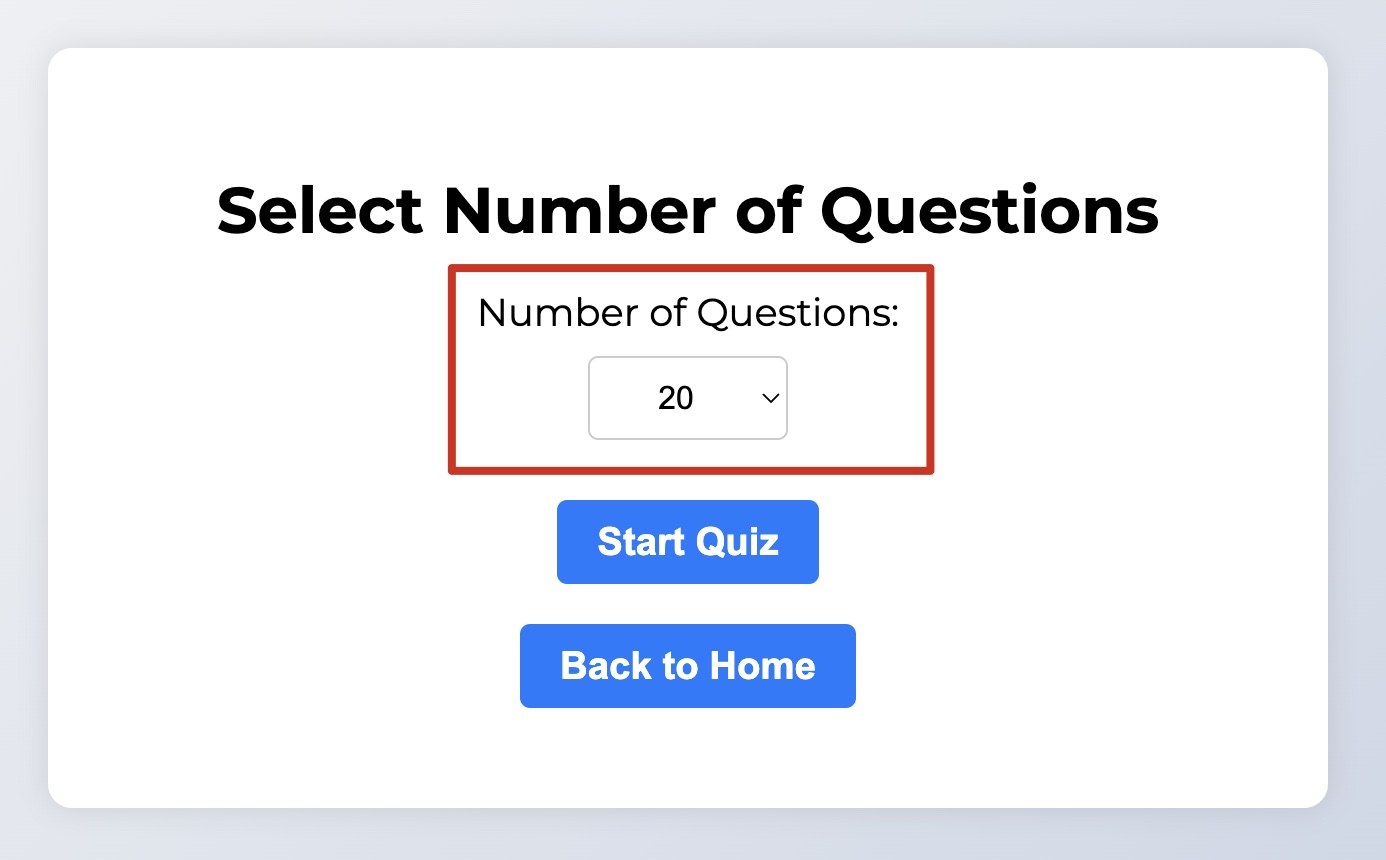
\includegraphics[width=0.5\textwidth]{start-quiz.jpg}
        \caption{問題数を選ぶ}
        \end{figure}

    \item 問題の意味が表示され、4つの選択肢から正しい単語を選択:\\
        例として、「a fact or object that helps to solve mysteries」という意味が表示され、選択肢の中から「clue」を選びます。クイズの状態は以下の図2に示す。
        
        \begin{figure}[H]
        \centering
        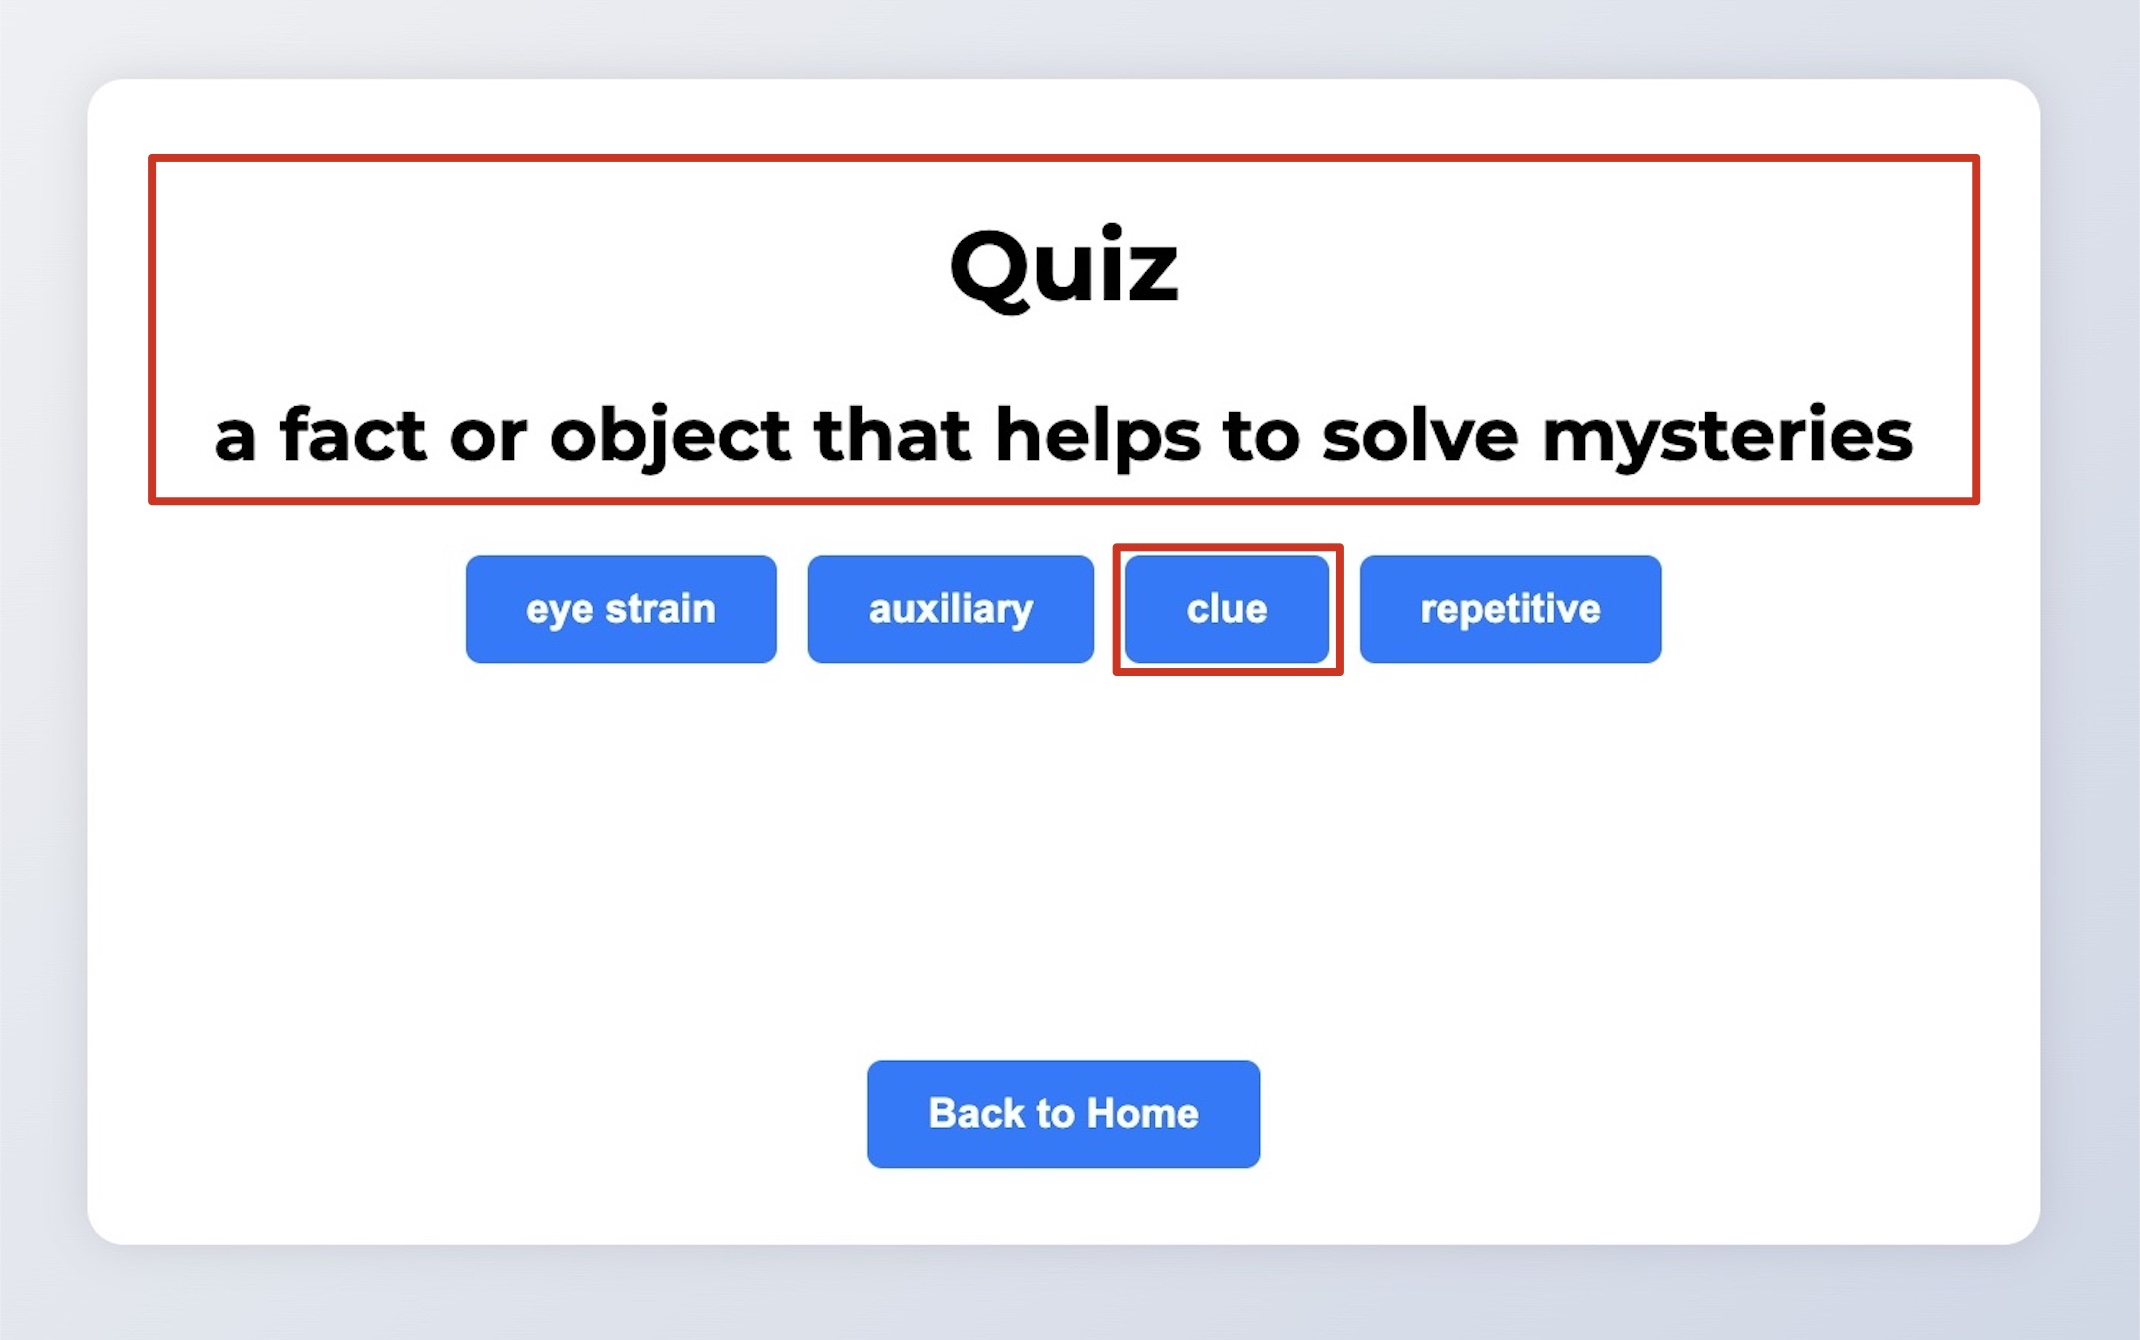
\includegraphics[width=0.5\textwidth]{question-display.jpg}
        \caption{クイズの状態}
        \end{figure}

    \item 回答後、「Next」ボタンをクリックして次の問題に進む:\\
        回答が正解の場合、「Correct!」、不正解の場合は「Incorrect! The correct answer is '単語'」というフィードバックが表示される。また、フィードバックと「Next」ボタンの状態を以下の図3に示す。
        
        \begin{figure}[H]
        \centering
        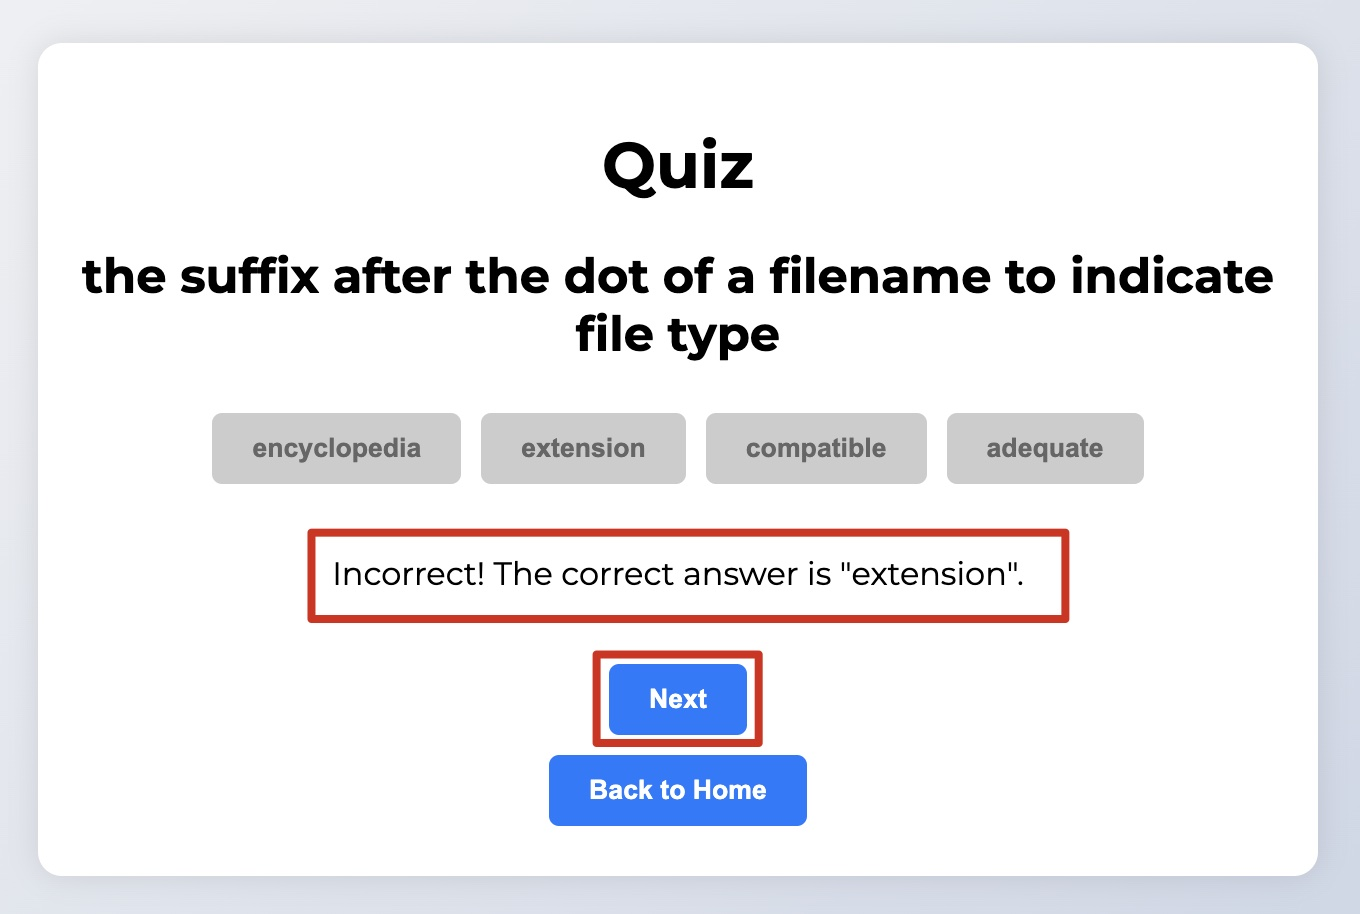
\includegraphics[width=0.5\textwidth]{score-display.jpg}
        \caption{回答が間違った場合}
        \end{figure}

    \item 選択した問題数を全て正しく回答しなければホームページに戻れない:\\
        クイズがまだ終わらない場合、ホームページに戻れなく、アラートが表示される。アラートが表示される状態を以下の図4に示す。
        
        \begin{figure}[H]
        \centering
        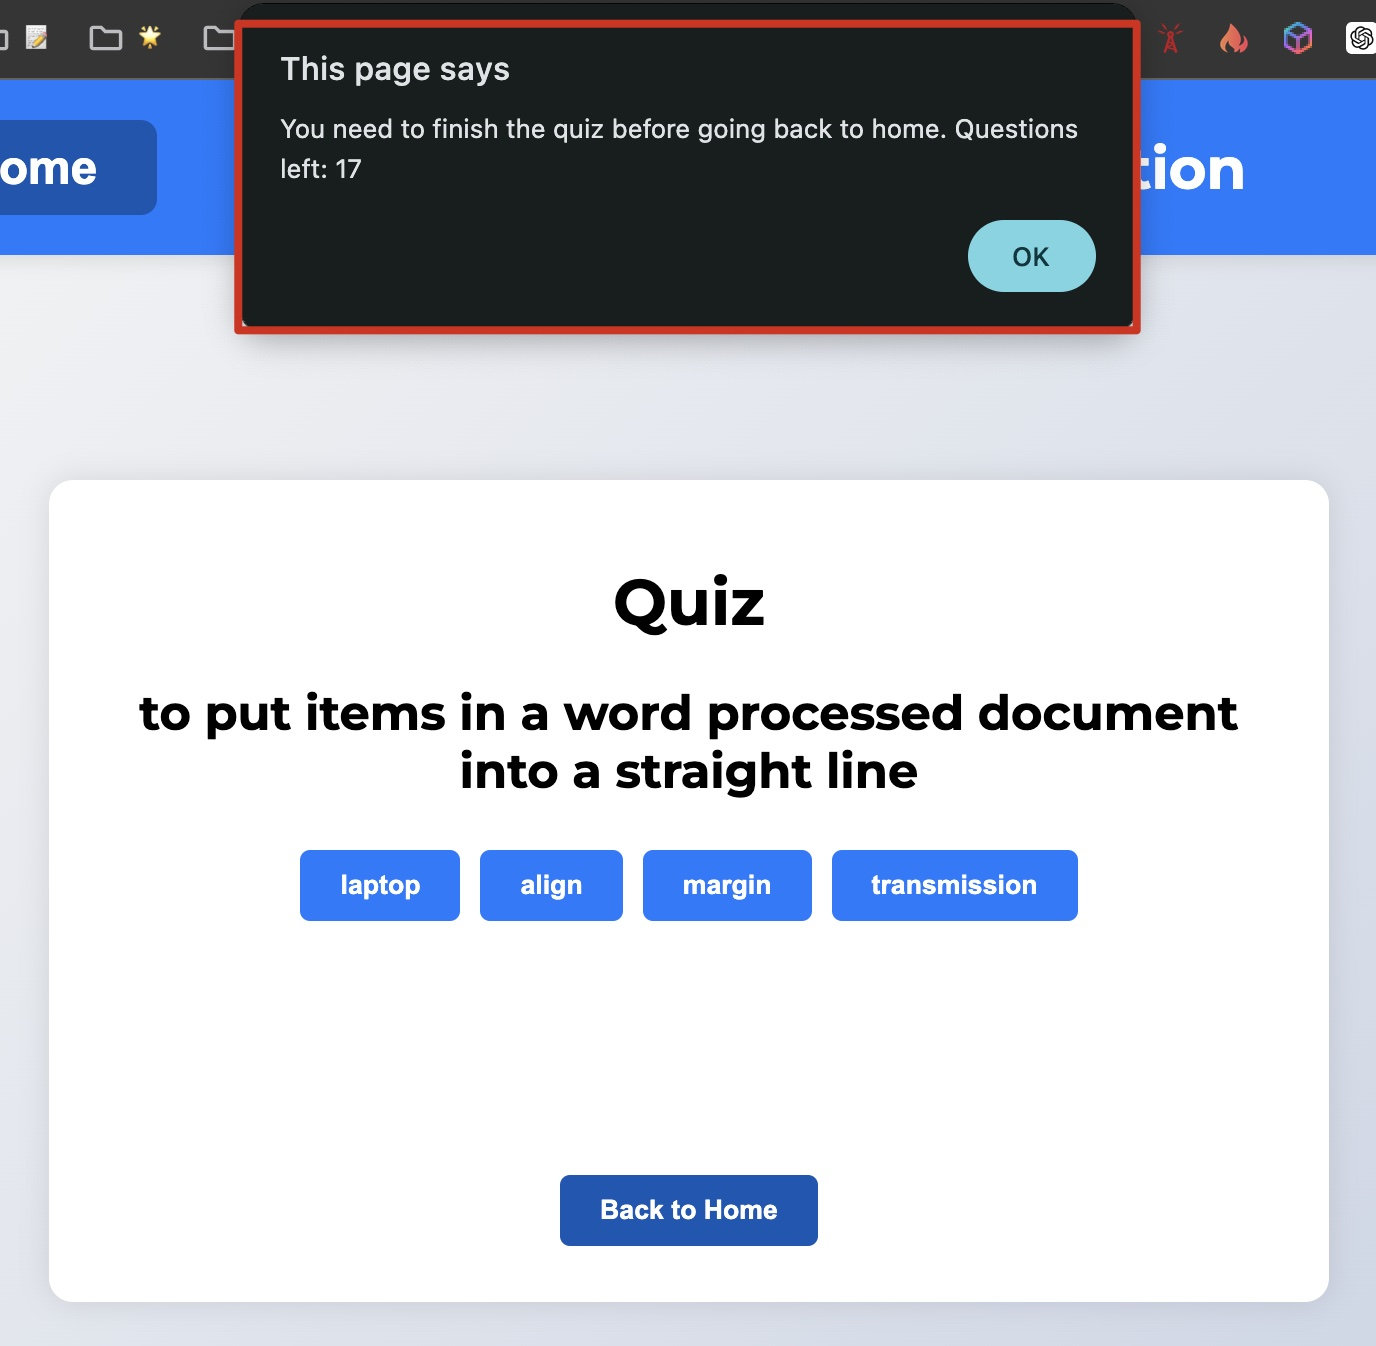
\includegraphics[width=0.5\textwidth]{alert-message.jpg}
        \caption{回答が間違った場合}
        \end{figure}

    \item クイズ終了後、スコアが表示される:\\
        全ての問題に回答後、総合スコアが表示される。スコアは「Score: 正解数/総問題数」の形式で表示される。クイズが終わると、スコアの表示状態を以下の図5に示す。
        
        \begin{figure}[H]
        \centering
        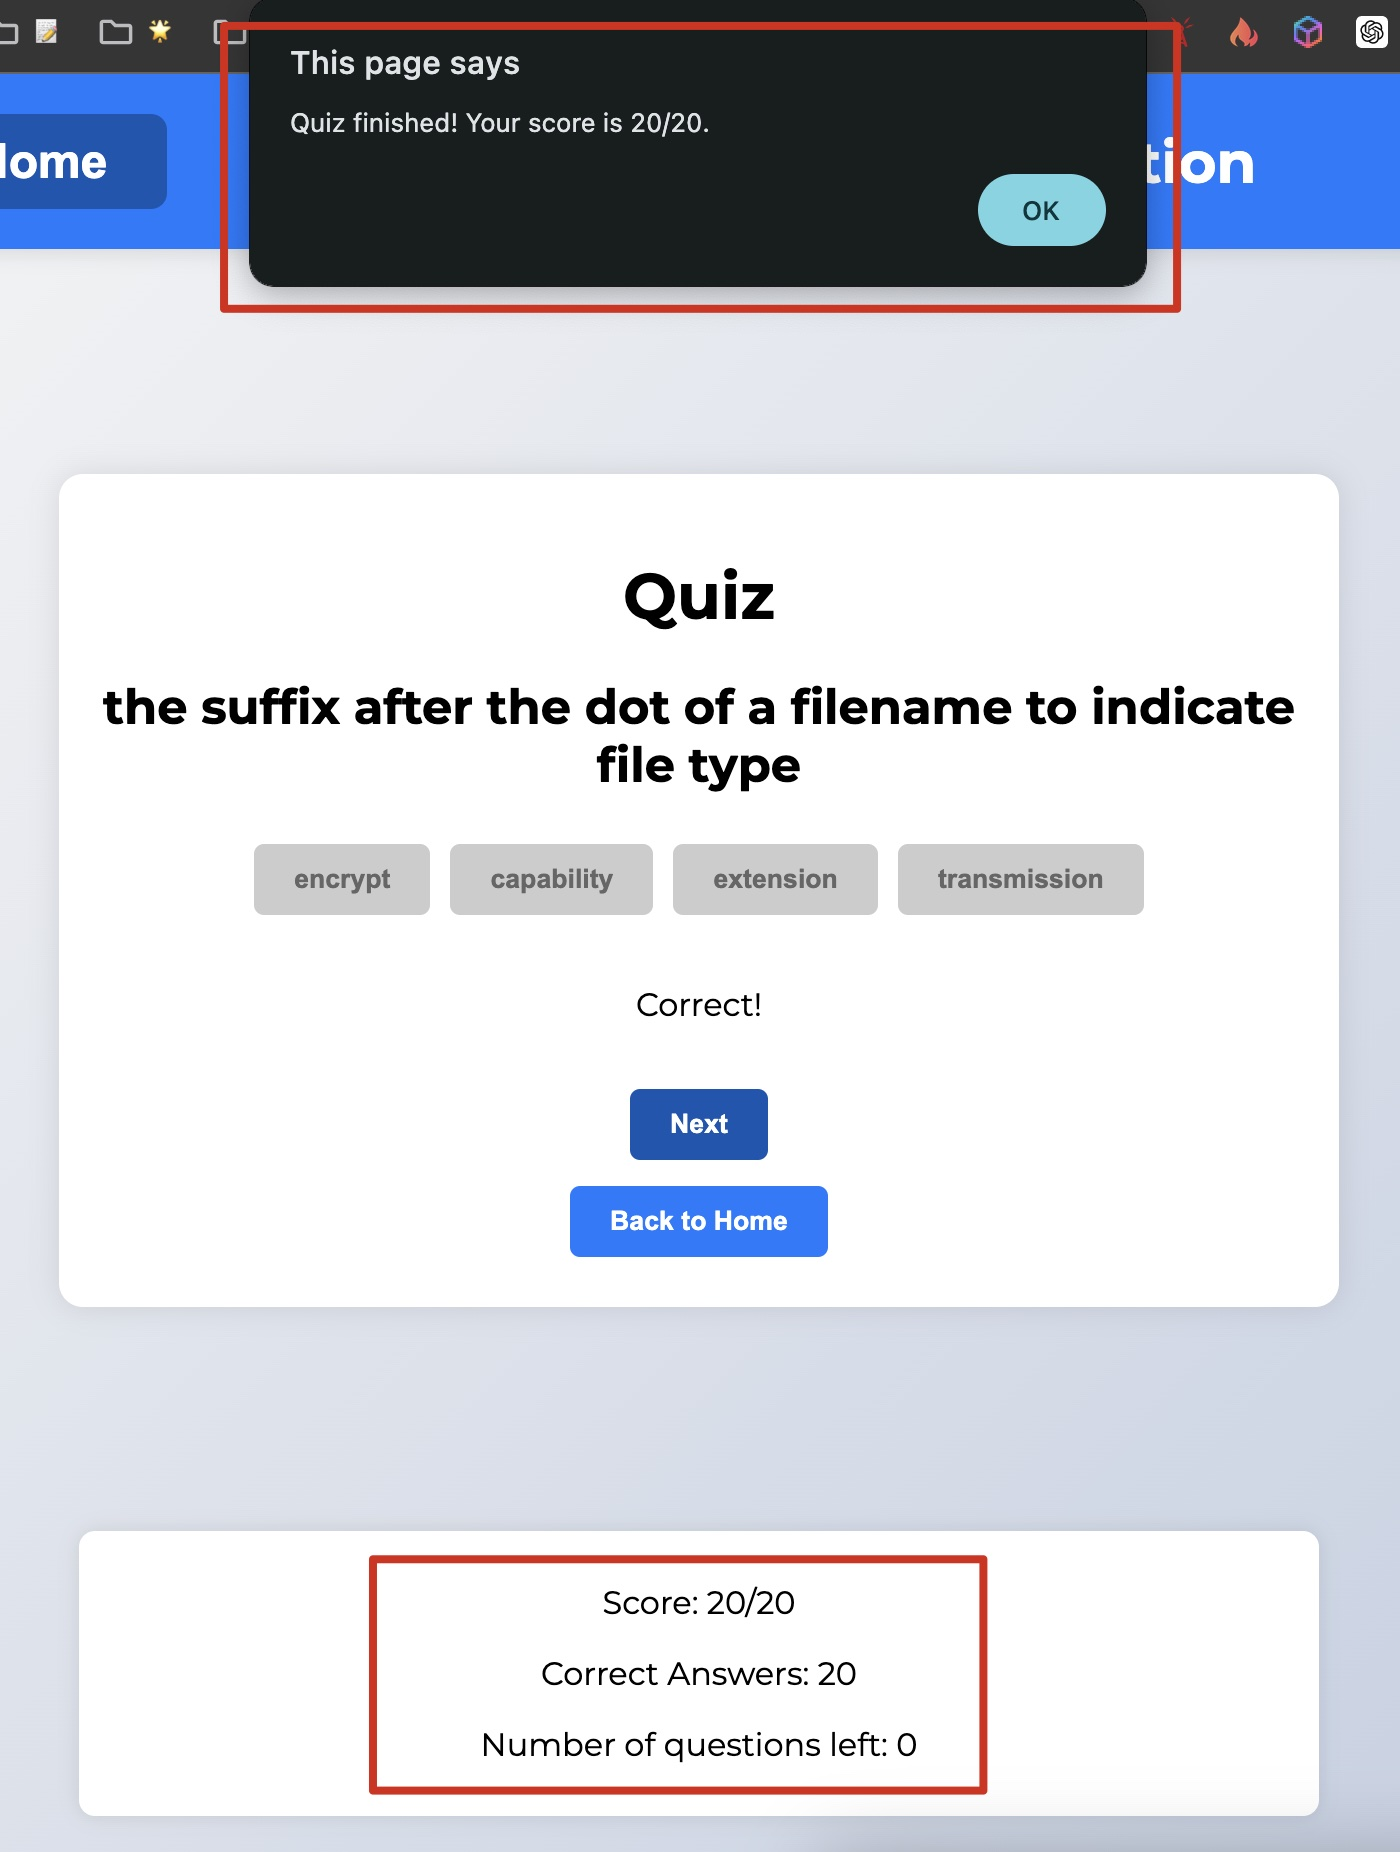
\includegraphics[width=0.5\textwidth]{score-display-2.jpg}
        \caption{スコアの表示}
        \end{figure}
\end{enumerate}

\subsection{フラッシュカードモードの実行例}

\begin{enumerate}
    \item ホーム画面で「Flashcards」ボタンをクリック:\\
        フラッシュカードモードが開始され、最初の単語とその意味が表示される。開始ボタンの状態を以下の図6に示す。
        
        \begin{figure}[H]
        \centering
        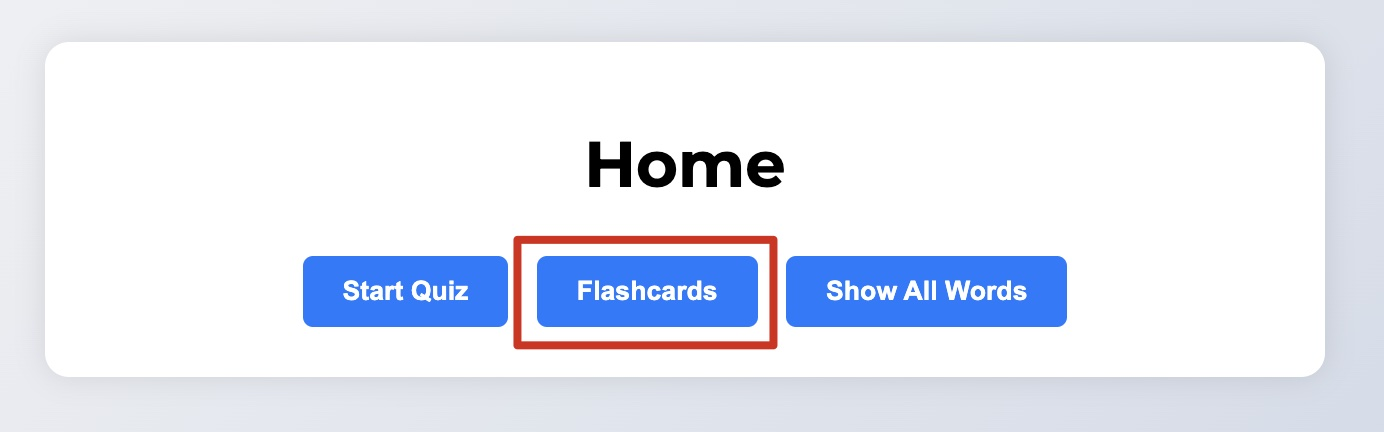
\includegraphics[width=0.5\textwidth]{flashcards-display.jpg}
        \caption{Flashcards開始}
        \end{figure}

    \item 「Show Answer」ボタンで答えを表示/非表示:\\
        学習者が「Show Answer」ボタンをクリックすると、単語の意味が表示され、もう一度クリックすると意味が隠れる。「Show Answer」と「Hide Answer」の状態を以下の図7に示す。
        
        \begin{figure}[H]
        \centering
        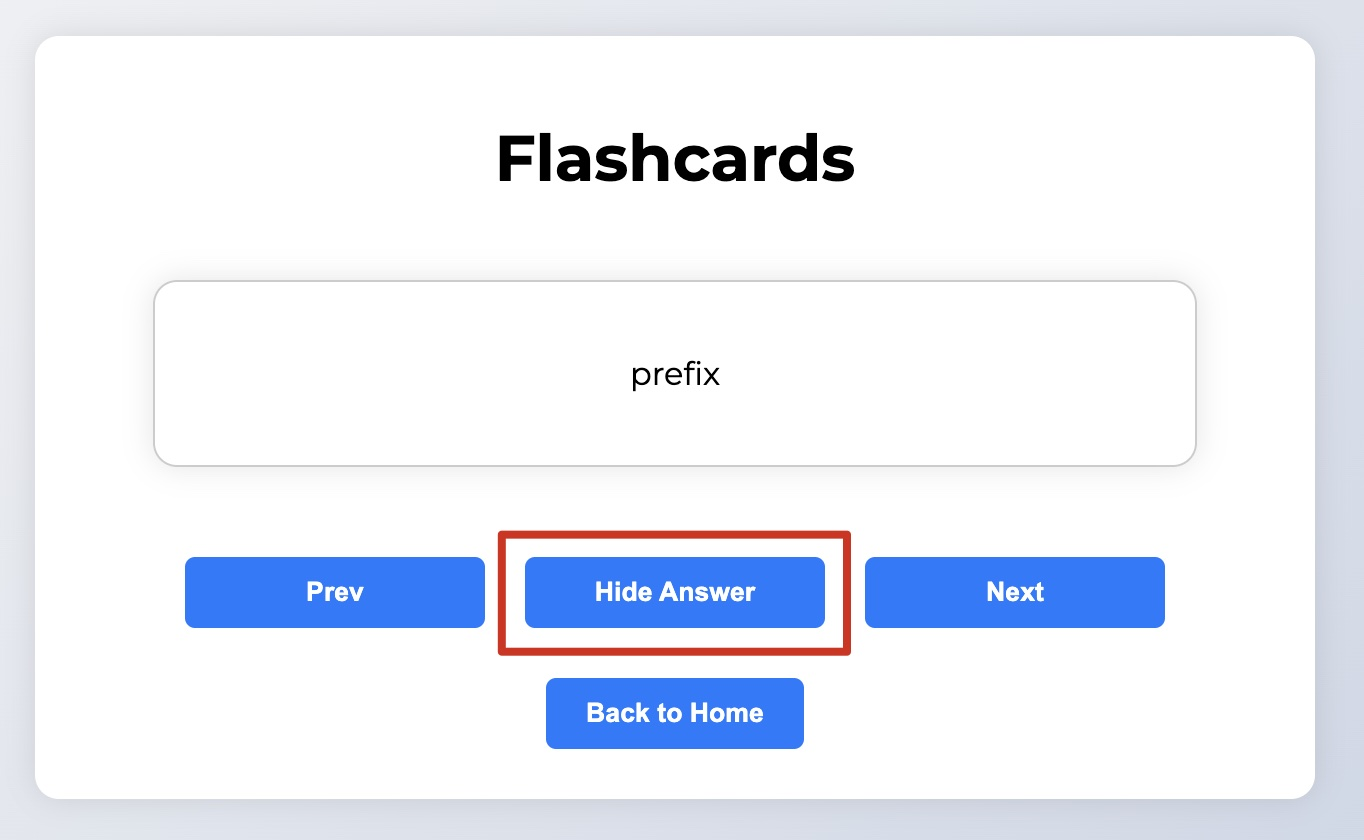
\includegraphics[width=0.5\textwidth]{show-hide-button.jpg}
        \caption{答えを表示する}
        \end{figure}

    \item 「Next」および「Prev」ボタンで前後のカードに移動:\\
        「Next」ボタンをクリックすると次のフラッシュカードに進み、「Prev」ボタンをクリックすると前のフラッシュカードに戻る。「Prev」と「Next」ボタンの状態を以下の図8に示す。
        
        \begin{figure}[H]
        \centering
        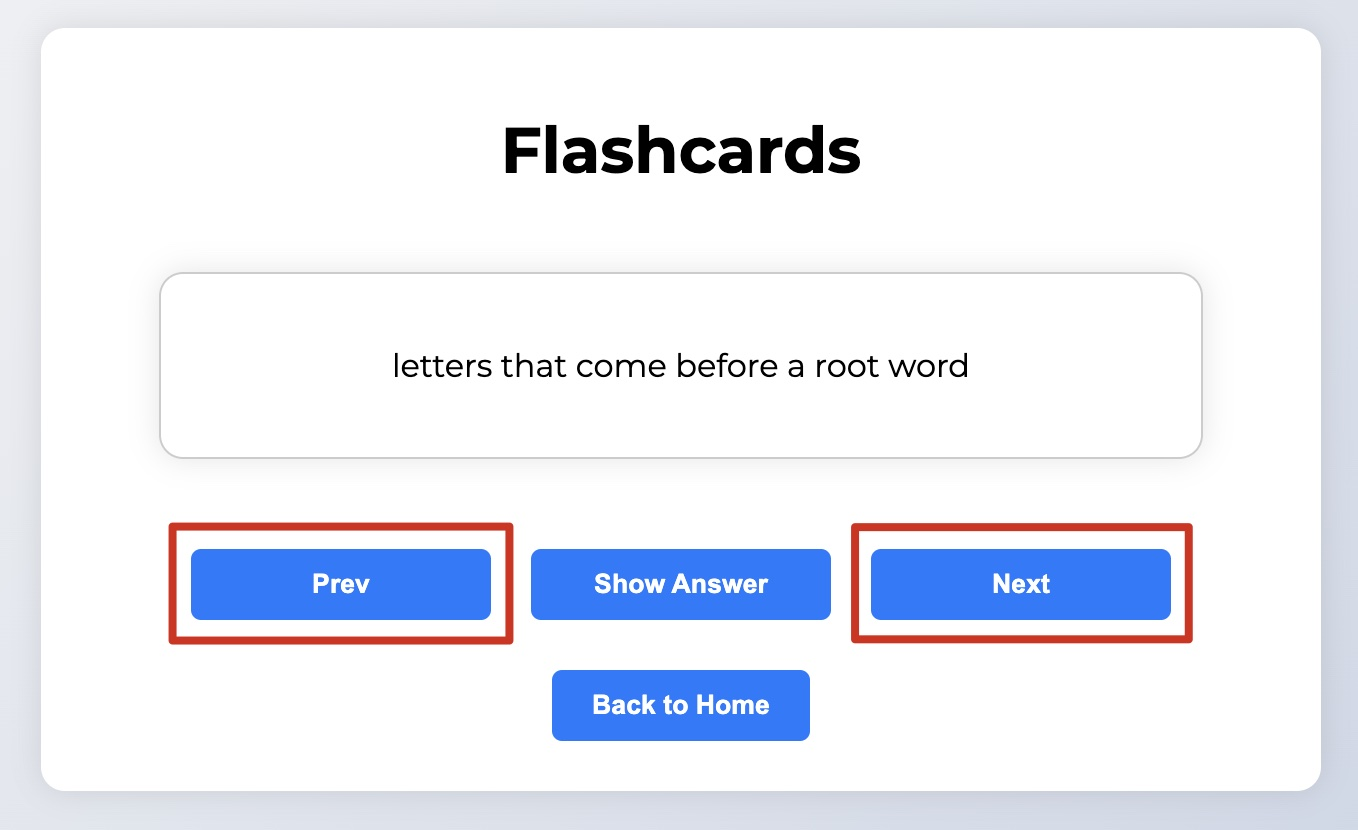
\includegraphics[width=0.5\textwidth]{prev-next-button.jpg}
        \caption{「Next」と「Previous」ボタン}
        \end{figure}
\end{enumerate}

\subsection{全単語リストの実行例}

\begin{enumerate}
    \item ホーム画面で「Show All Words」ボタンをクリック:\\
        全単語リストが表示される。PWT-R 100-word listの全単語とその意味が一覧表示される。単語一覧の状態を以下の図9に示す。
        
        \begin{figure}[H]
        \centering
        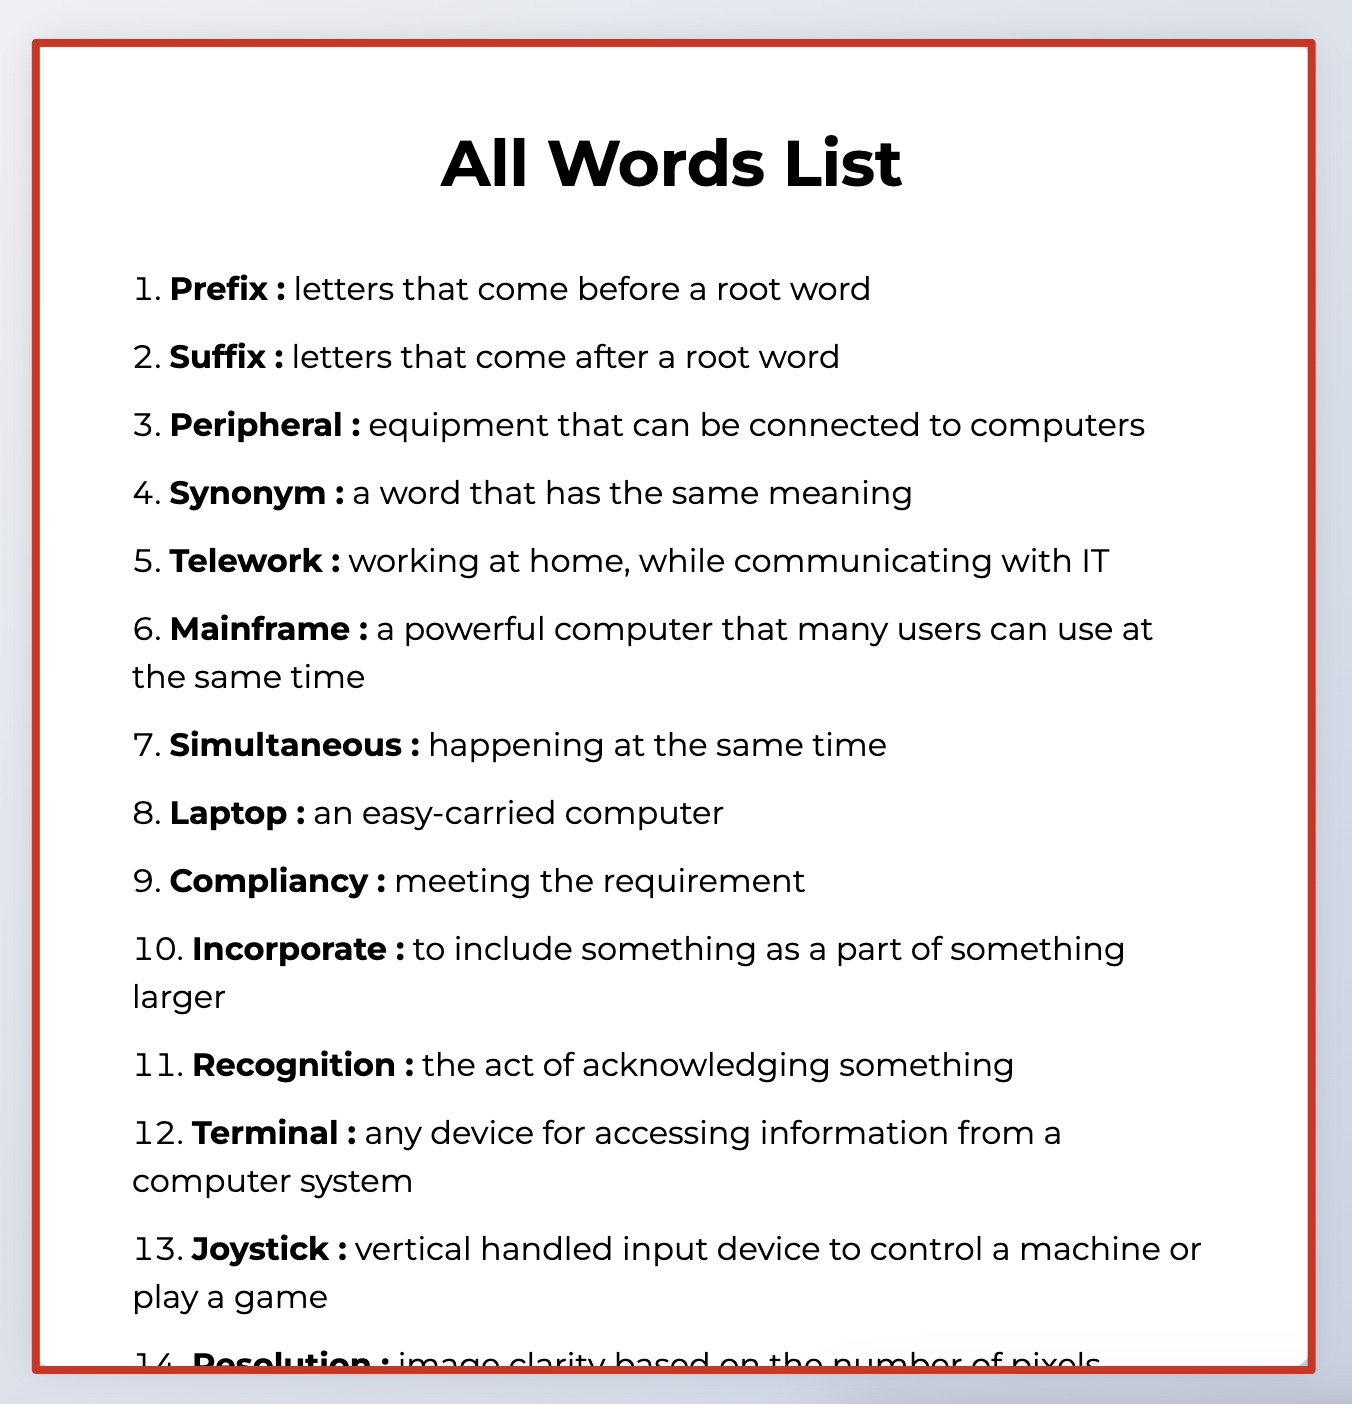
\includegraphics[width=0.5\textwidth]{show-all-words.jpg}
        \caption{全ての単語一覧}
        \end{figure}

    \item 学習者は全ての単語とその意味を確認:\\
        学習者はスクロールしてリスト全体を確認し、復習に役立てることができる。\\

    \item 「Back to Home」ボタンをクリックしてホーム画面に戻る:\\
        学習者が「Back to Home」ボタンをクリックすると、ホーム画面に戻る。一番下までスクロールすると、「Back to Home」ボタンが表示される。ボタンの状態を以下の図10に示す。
        
        \begin{figure}[H]
        \centering
        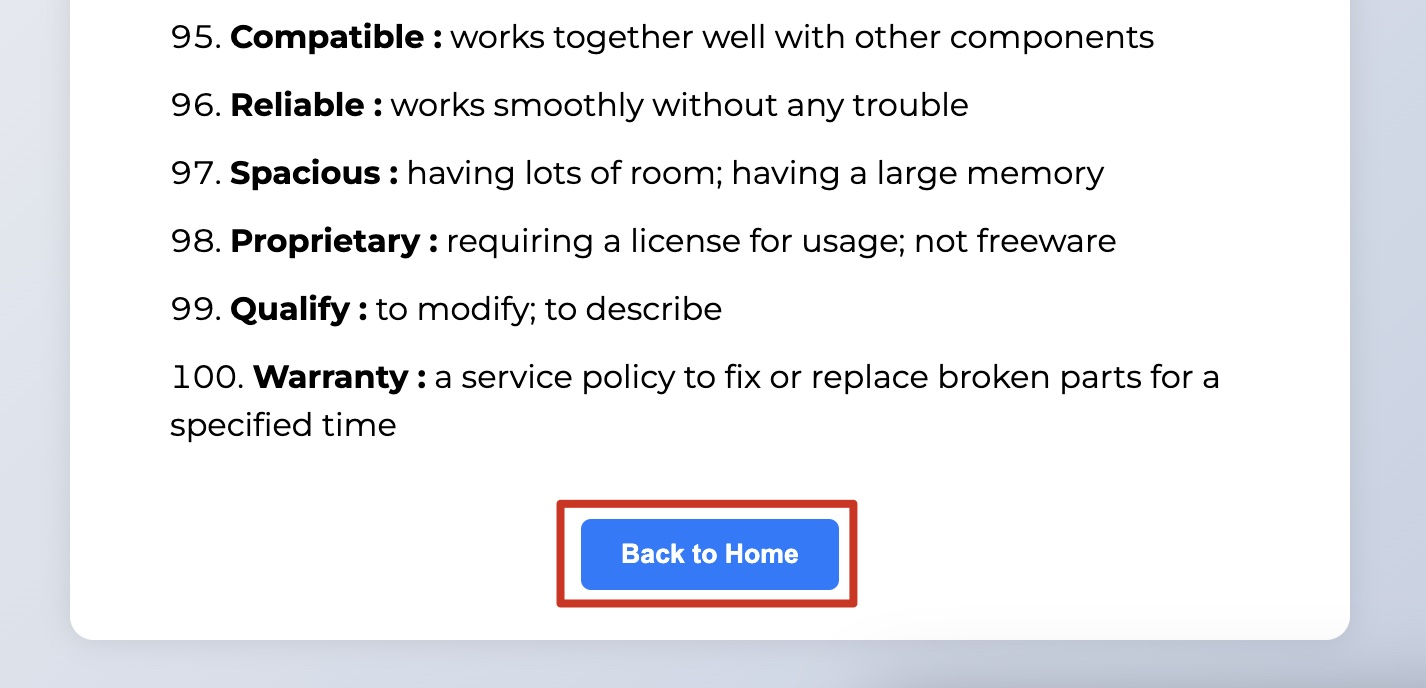
\includegraphics[width=0.5\textwidth]{all-words-back-to-home.jpg}
        \caption{「Back to Home」ボタン}
        \end{figure}
\end{enumerate}

\newpage
\section{結論}

WordMaster: PWT-R Editionは、英語のPWT-R 100-word listの試験に向けて効果的に学習をサポートするアプリである。クイズとフラッシュカードを通じて、学習者は楽しく語彙力を強化することができると考えられる。また、問題数を選択できる機能や、全単語リストを表示する機能により、学習者は自分のペースで学習を進めることができる。
今後は、さらなる機能追加の改善を図り、より使いやすいアプリに進化させる予定である。追加できる機能としては、他のクイズ形式(穴埋めやマッチングなど)の追加や、単語の発音を聞く機能の追加などが考えられる。
また、アカウント管理機能とスコアのランキング機能を追加することで、学習者同士の競争を促し、学習意欲を高めることができると考えられる。

\end{document}